% ==========================================
% CHƯƠNG 4: THỰC NGHIỆM VÀ ĐÁNH GIÁ KẾT QUẢ
% ==========================================
% Biến số liệu, cập nhật sau khi có kết quả mới
\newcommand{\Ntest}{232}           % N test samples (cấp độ đa giác)
\newcommand{\Ntestimg}{187}        % N test images  (merged mask, UNet)
\newcommand{\Ntrain}{1\,493}       % N train samples
\newcommand{\Nval}{187}            % N val samples

% Bộ dữ liệu FracAtlas (đánh giá bổ sung sau khi huấn luyện lại trên miền dữ liệu khác)
\newcommand{\NtestFA}{92}          % N test samples FracAtlas (cấp độ đa giác)
\newcommand{\NtestimgFA}{72}       % N test images FracAtlas (image-level)
\newcommand{\NtrainFA}{730}        % N train samples FracAtlas (cấp độ đa giác)
\newcommand{\NvalFA}{95}           % N val samples FracAtlas (cấp độ đa giác)

% ==========================================
\chapter{THỰC NGHIỆM VÀ ĐÁNH GIÁ KẾT QUẢ}
\label{Chapter4}

Chương này trình bày phần thực nghiệm của khóa luận trên hai bộ dữ liệu BTXRD và FracAtlas. Để dễ theo dõi hơn, nội dung được chia theo từng nhóm vấn đề. Mục~\ref{sec:thiet_lap} nói về dữ liệu và cấu hình thực nghiệm. Mục~\ref{sec:danh_gia_hieu_nang} trình bày các kết quả phân đoạn chính, gồm so sánh với U-Net, Attention U-Net, SAM-Med2D, ảnh hưởng của độ phân giải và độ ổn định khi câu nhắc bị lệch trong phạm vi bài toán. Mục~\ref{sec:ablation_study} tóm tắt các kết luận quan trọng từ nghiên cứu loại bỏ thành phần, kiểm chứng chéo và phân tích theo đặc tính tổn thương; phần số liệu đầy đủ được để ở Phụ lục~\ref{AppendixA}. Cuối cùng, Mục~\ref{sec:product_overview} trình bày thử nghiệm mở rộng với Gatekeeper và luồng xử lý hai giai đoạn; các bảng chi tiết nằm ở Phụ lục~\ref{AppendixB}.

% ============================================================
% PHẦN I, ĐÓNG GÓP 1: Nghiên cứu kiến trúc PGA-UNet
% ============================================================

% ------------------------------------------------------------
\section{Thiết lập môi trường thực nghiệm}
\label{sec:thiet_lap}
% ------------------------------------------------------------

Phần này trình bày về tập dữ liệu, cách phân chia dữ liệu thành các tập huấn luyện và đánh giá, cấu hình phần cứng và các siêu tham số huấn luyện. Đây là cơ sở để tiến hành thực nghiệm cũng như đánh giá kết quả ở những mục sau.

\subsection{Hai bộ dữ liệu ảnh X-quang và tiền xử lý đầu vào}
\label{subsec:dataset}

Khóa luận sử dụng hai bộ dữ liệu X-quang xương công khai và độc lập là BTXRD~\cite{btxrd2024}(Bone Tumor X-Ray Dataset) và FracAtlas~\cite{fracatlas2023}. BTXRD tập trung vào khối u xương, còn FracAtlas tập trung vào gãy xương ở nhiều vị trí khác nhau. Việc dùng cả hai bộ dữ liệu giúp mô hình được kiểm tra trên hai dạng tổn thương khác nhau: một bên là vùng tổn thương có hình dạng phức tạp hơn, một bên là các đường gãy thường nhỏ và mảnh hơn.

Dữ liệu dùng cho bài toán phân đoạn chỉ gồm ảnh bệnh lý có mặt nạ ở cấp độ điểm ảnh.
\begin{table}[H]
    \centering
    \caption{Thống kê phân bố hai bộ dữ liệu dùng trong thực nghiệm}
    \label{tab:dataset_stats}
    \renewcommand{\arraystretch}{1.3}
    \setlength{\tabcolsep}{4pt}
    \small
    \begin{tabular}{|c|p{2.1cm}|c|p{2.5cm}|p{4.8cm}|}
        \hline
        \textbf{Bộ dữ liệu} & \textbf{Phân chia} & \textbf{Số ảnh} & \textbf{Số mẫu đa giác} & \textbf{Ghi chú} \\
        \hline
        \multirow{3}{*}{BTXRD}
        & Huấn luyện & \Ntrain & 1847 & Ảnh khối u xương có mặt nạ phân đoạn. \\
        \cline{2-5}
        & Xác thực & \Nval & 239 & Dùng để lựa chọn mô hình. \\
        \cline{2-5}
        & Kiểm thử & \Ntestimg & \Ntest & Một số ảnh chứa từ hai vùng tổn thương trở lên. \\
        \hline
        \multirow{3}{*}{FracAtlas}
        & Huấn luyện & 573 & \NtrainFA & Ảnh gãy xương có mặt nạ phân đoạn. \\
        \cline{2-5}
        & Xác thực & 72 & \NvalFA & Dùng để lựa chọn mô hình. \\
        \cline{2-5}
        & Kiểm thử & \NtestimgFA & \NtestFA & Trung bình khoảng 1,28 vùng tổn thương trên mỗi ảnh. \\
        \hline
    \end{tabular}
\end{table}

FracAtlas có 917 mẫu đa giác được dùng trong thực nghiệm, khá gần với 922 vùng gãy xương được công bố trong bộ dữ liệu gốc~\cite{fracatlas2023}. Phần chênh lệch nhỏ hơn 1\% chủ yếu do một số đa giác quá nhỏ hoặc lỗi định dạng bị loại ra khi chuẩn hóa dữ liệu. So với BTXRD, FracAtlas có ít dữ liệu huấn luyện hơn, nên cũng giúp kiểm tra thêm khả năng học của PGA-UNet trong điều kiện dữ liệu hạn chế hơn.

Phần tiền xử lý được áp dụng giống nhau cho cả hai bộ dữ liệu. Ảnh X-quang được chuẩn hóa về kích thước $512\times512$ hoặc $256\times256$. Mặt nạ nhị phân được tạo từ tọa độ đa giác trong chú thích và cũng được biến đổi theo đúng quy trình đó. Tương tự, bản đồ nhiệt câu nhắc được chuẩn hóa theo cùng cách để đồng bộ với ảnh đầu vào. Dữ liệu sau tiền xử lý được dùng thống nhất trong huấn luyện, suy luận và lúc trực quan hóa kết quả.

Việc phân chia tập huấn luyện, xác thực và kiểm thử được thực hiện ở cấp độ ảnh: các đa giác thuộc cùng một ảnh luôn được giữ trong cùng một tập để tránh rò rỉ dữ liệu ở cấp độ vùng tổn thương. Khóa luận chưa xác nhận việc phân chia ở cấp độ bệnh nhân hoặc lượt chụp (nhiều ảnh của cùng một bệnh nhân, nếu có, có thể rơi vào các tập khác nhau), do siêu dữ liệu công khai của BTXRD và FracAtlas không cung cấp mã định danh bệnh nhân đầy đủ để kiểm tra. Đây là một giới hạn về khả năng kiểm chứng rò rỉ dữ liệu, được nêu lại tại Mục~\ref{sec:han_che}, Chương~\ref{Chapter5}.
% ------------------------------------------------------------
\subsection{Mô hình so sánh và cấu hình huấn luyện}
\label{subsec:models_compared}

PGA-UNet được so sánh với U-Net, Attention U-Net và SAM-Med2D. Trong đó, U-Net~\cite{ronneberger2015unet} và Attention U-Net~\cite{oktay2018attentionunet} đóng vai trò mô hình cơ sở tự động, không nhận câu nhắc không gian. SAM-Med2D~\cite{2023-SAMMed2D-Cheng} là mô hình nền tảng có thể nhận hộp giới hạn và được đánh giá ở hai chế độ là chưa tinh chỉnh và đã tinh chỉnh trên từng bộ dữ liệu. PGA-UNet là mô hình đề xuất của khóa luận, sử dụng bản đồ nhiệt Gaussian kết hợp với PSG và CAD.

U-Net, Attention U-Net và PGA-UNet được huấn luyện từ đầu riêng biệt trên BTXRD và FracAtlas. SAM-Med2D ở chế độ chưa tinh chỉnh sử dụng trực tiếp trọng số tiền huấn luyện; ở chế độ đã tinh chỉnh, lớp thích ứng và bộ giải mã được cập nhật trên từng bộ dữ liệu. Kết quả so sánh với SAM-Med2D được trình bày tại Mục~\ref{subsec:sam_comparison}; ảnh hưởng của độ phân giải và câu nhắc lệch trong phạm vi bài toán được phân tích tại Mục~\ref{subsec:resolution_prompt}.

\paragraph{Cấu hình huấn luyện.}
Các mô hình được triển khai bằng PyTorch và huấn luyện trong môi trường Kaggle sử dụng GPU NVIDIA Tesla T4 với 16 GB bộ nhớ. Các thực nghiệm trên hai bộ dữ liệu sử dụng cùng quy trình tiền xử lý và hàm mất mát. Đối với các mô hình huấn luyện từ đầu, hàm mất mát kết hợp entropy chéo nhị phân và Dice được sử dụng để xử lý sự mất cân bằng giữa vùng tổn thương và vùng nền:
\begin{equation}
    \mathcal{L}_{\mathrm{total}}
    = \mathcal{L}_{\mathrm{BCE}}
    + \mathcal{L}_{\mathrm{Dice}}.
    \label{eq:loss_seg}
\end{equation}

Các mô hình sử dụng kích thước lô 4, bộ tối ưu AdamW, tốc độ học ban đầu $10^{-4}$ và hệ số suy giảm trọng số $10^{-4}$. Việc huấn luyện và lựa chọn mô hình được thực hiện nhất quán trên toàn bộ thực nghiệm.

Đối với PGA-UNet, hệ số điều biến tại bốn tầng giải mã là $w_l=\{1{,}0;\,0{,}7;\,0{,}4;\,0{,}2\}$, hệ số pha trộn học được của CAD được khởi tạo bằng $\alpha_{\mathrm{CAD}}=0{,}3$ (tương ứng đại lượng $\alpha^{l}_{\mathrm{CAD}}$ tại Phương trình~\eqref{eq:conditioned_gate}, Chương~\ref{Chapter3}) và tham số cổng PSG được khởi tạo với $\alpha_{\mathrm{gate}}=0{,}1$. Bản đồ nhiệt Gaussian sử dụng cửa sổ lọc $k=31$; hộp giới hạn được mở rộng thêm 5 điểm ảnh ở mỗi cạnh. Các giá trị này được áp dụng thống nhất trong các phép đánh giá của khóa luận. Do chúng được giữ theo đơn vị điểm ảnh cho cả ảnh $256\times256$ và $512\times512$, mức độ làm mềm và biên mở rộng tương đối không hoàn toàn giống nhau giữa hai độ phân giải; điểm này cần được lưu ý khi diễn giải kết quả tại Mục~\ref{subsec:resolution_prompt}.
% ------------------------------------------------------------
\subsection{Phương pháp đánh giá cấp độ ảnh}
\label{subsec:image_level_eval}

Một ảnh kiểm thử có thể chứa nhiều vùng tổn thương, và mỗi vùng được chú thích bằng một đa giác riêng.

\begin{enumerate}
    \item \textbf{Hợp nhất nhãn gốc:} Với ảnh chứa $K\geq1$ vùng tổn thương, các mặt nạ nhị phân $\{G_1,G_2,\ldots,G_K\}$ được hợp nhất thành một mặt nạ duy nhất:
    \begin{equation}
        M_{\mathrm{GT}}=\bigcup_{k=1}^{K}G_k.
        \label{eq:gt_union}
    \end{equation}

    \item \textbf{Kết hợp dự đoán:} Mô hình suy luận riêng với từng hộp giới hạn $\mathbf{B}_k$ để sinh các mặt nạ xác suất $\{\hat{P}_1,\hat{P}_2,\ldots,\hat{P}_K\}$. Các kết quả được kết hợp để tạo ra tập hợp các mặt nạ nhị phân:
    \begin{equation}
        \hat{M}_{\mathrm{max}}(x,y)
        =\max_{1\leq k\leq K}\hat{P}_k(x,y).
        \label{eq:pred_max_merge}
    \end{equation}
    Mặt nạ nhị phân cuối cùng được xác định bởi
    $\hat{M}_{\mathrm{pred}}
    =\mathbf{1}[\hat{M}_{\mathrm{max}}\geq0.5]$.

    \item \textbf{Tính chỉ số cấp độ ảnh:} Các chỉ số đánh giá được tính một lần giữa $\hat{M}_{\mathrm{pred}}$ và $M_{\mathrm{GT}}$. Chẳng hạn, Dice cấp độ ảnh được xác định bởi:
    \begin{equation}
        \mathrm{Dice}_{\mathrm{img}}
        =\frac{2|M_{\mathrm{GT}}\cap\hat{M}_{\mathrm{pred}}|}
        {|M_{\mathrm{GT}}|+|\hat{M}_{\mathrm{pred}}|}.
        \label{eq:dice_img}
    \end{equation}
\end{enumerate}

Kết quả cuối cùng được lấy trung bình trên toàn bộ ảnh kiểm thử của từng bộ dữ liệu. Cách đánh giá này bảo đảm mỗi ảnh chỉ đóng góp một lần vào kết quả tổng hợp, không phụ thuộc vào số vùng tổn thương.

Đối với ảnh có nhiều vùng tổn thương, số lượng và vị trí hộp giới hạn $\mathbf{B}_k$ được suy ra trực tiếp từ số vùng và tọa độ của mặt nạ nhãn gốc. Nói cách khác, các kết quả ở mục này không đánh giá một hệ thống phát hiện--phân đoạn hoàn chỉnh phải tự xác định số lượng và vị trí tổn thương trên ảnh chưa có nhãn, mà đánh giá chất lượng phân đoạn khi thông tin định vị sơ bộ đã được cung cấp.

HD95 không xác định về mặt toán học khi $M_{\mathrm{GT}}$ hoặc $\hat{M}_{\mathrm{pred}}$ rỗng, tình huống có thể xảy ra với các mô hình có tỷ lệ dự đoán rỗng cao, chẳng hạn U-Net trên một số nhóm phụ tại Phụ lục~\ref{AppendixA}. Vì vậy, các giá trị HD95 trong khóa luận được tính theo một quy ước bổ sung thay vì công thức chuẩn áp dụng trực tiếp cho mọi trường hợp: nếu cả hai mặt nạ đều rỗng, HD95 được gán giá trị 0; nếu chỉ một trong hai mặt nạ rỗng, HD95 được gán giá trị phạt cố định bằng kích thước cạnh ảnh (256 hoặc 512 điểm ảnh, tùy độ phân giải đánh giá). Không có mẫu nào bị loại khỏi phép tính trung bình.
% ============================================================
\section{Đánh giá hiệu năng kiến trúc PGA-UNet}
\label{sec:danh_gia_hieu_nang}
% ============================================================

Mục này đánh giá hiệu năng của PGA-UNet theo ba hướng chính: so với các mô hình phân đoạn tự động, so với mô hình nền tảng SAM-Med2D và theo ảnh hưởng của độ phân giải đầu vào. Ngoài độ chính xác phân đoạn, phần này cũng kiểm tra mức độ ổn định của mô hình khi câu nhắc bị lệch trong phạm vi bài toán.

% ------------------------------------------------------------
\subsection{So sánh với các mô hình cơ sở}
\label{subsec:baseline_comparison}
% ------------------------------------------------------------

Thực nghiệm đầu tiên so sánh PGA-UNet với U-Net và Attention U-Net trên cả BTXRD và FracAtlas. Trong so sánh này, U-Net và Attention U-Net hoạt động hoàn toàn tự động, còn PGA-UNet nhận thêm câu nhắc là hộp giới hạn Bao trọn.

Cả ba mô hình được huấn luyện từ đầu riêng biệt trên từng bộ dữ liệu với cùng kích thước đầu vào và được đánh giá ở cấp độ ảnh. So sánh này nhằm xác định lợi ích tổng thể của phương pháp phân đoạn có hướng dẫn bằng câu nhắc so với các mô hình cơ sở không sử dụng câu nhắc; đây không phải phép so sánh cùng điều kiện đầu vào, nên không được dùng để kết luận về tính mới của riêng kiến trúc PGA-UNet. Đóng góp cụ thể của PSG và CAD, tách biệt khỏi lợi ích của việc có câu nhắc, được kiểm chứng bằng các cấu hình đối sánh cùng nhận câu nhắc (U-Net+Concat, U-Net+PSG, U-Net+CAD) tại Mục~\ref{sec:ablation_study} và Phụ lục~\ref{AppendixA}.

\begin{table}[H]
    \centering
    \caption{So sánh PGA-UNet với các mô hình cơ sở trên BTXRD ở độ phân giải $512\times512$ (N=\Ntestimg~ảnh)}
    \label{tab:baseline_comparison}
    \renewcommand{\arraystretch}{1.3}
    \resizebox{\textwidth}{!}{%
    \begin{tabular}{|l|c|c|c|c|c|c|}
        \hline
        \textbf{Mô hình} & \textbf{Dice↑} & \textbf{IoU↑} & \textbf{Precision↑} & \textbf{Recall↑} & \textbf{HD95↓ (px)} & \textbf{CBL↑} \\
        \hline
        U-Net & 0.4740 & 0.3741 & 0.5847 & 0.5341 & 144.37 & 0.5709 \\
        \hline
        Attention U-Net & 0.4122 & 0.3291 & 0.5988 & 0.4065 & 136.75 & 0.5701 \\
        \hline
        \textbf{PGA-UNet (Bao trọn)}
        & \textbf{0.8607}
        & \textbf{0.7630}
        & \textbf{0.8476}
        & \textbf{0.8882}
        & \textbf{12.12}
        & \textbf{0.9564} \\
        \hline
    \end{tabular}%
    }
\end{table}

\begin{table}[H]
    \centering
    \caption{So sánh PGA-UNet với các mô hình cơ sở trên FracAtlas ở độ phân giải $512\times512$ (N=\NtestimgFA~ảnh)}
    \label{tab:fracatlas_baseline}
    \renewcommand{\arraystretch}{1.3}
    \resizebox{\textwidth}{!}{%
    \begin{tabular}{|l|c|c|c|c|c|c|}
        \hline
        \textbf{Mô hình} & \textbf{Dice↑} & \textbf{IoU↑} & \textbf{Precision↑} & \textbf{Recall↑} & \textbf{HD95↓ (px)} & \textbf{CBL↑} \\
        \hline
        U-Net & 0.3831 & 0.2836 & 0.4387 & 0.4642 & 136.82 & 0.4628 \\
        \hline
        Attention U-Net & 0.2467 & 0.1816 & 0.4754 & 0.3006 & 186.46 & 0.3902 \\
        \hline
        \textbf{PGA-UNet (Bao trọn)}
        & \textbf{0.8169}
        & \textbf{0.6953}
        & \textbf{0.7645}
        & \textbf{0.8975}
        & \textbf{7.45}
        & \textbf{0.9546} \\
        \hline
    \end{tabular}%
    }
\end{table}

Trong thiết lập phân đoạn có hướng dẫn bằng hộp giới hạn, PGA-UNet cho kết quả cao hơn các mô hình cơ sở trên cả hai bộ dữ liệu. So với U-Net, Dice tăng 0,3867 trên BTXRD và 0,4338 trên FracAtlas; HD95 cũng giảm mạnh từ 144,37 xuống 12,12 và từ 136,82 xuống 7,45 điểm ảnh. CBL ở cả hai bộ dữ liệu đều lớn hơn 0,95. Tóm lại, khi đã có thông tin định vị sơ bộ thì mô hình chạy ổn hơn hẳn và không còn lệch nhiều như các mô hình tự động.

Attention U-Net trong thí nghiệm này không cải thiện được Dice so với U-Net. Còn PGA-UNet thì tăng cùng lúc nhiều chỉ số như Dice, IoU, Recall, HD95 và CBL trong so sánh giữa mô hình có câu nhắc và mô hình không dùng câu nhắc. Chỗ này chủ yếu cho thấy việc có thêm thông tin định vị từ hộp giới hạn là hữu ích với bài toán đang xét. Phần đóng góp riêng của từng thành phần kiến trúc sẽ được tách ra để phân tích kỹ hơn ở Mục~\ref{sec:ablation_study} và Phụ lục~\ref{AppendixA}. Hình~\ref{fig:vis_pga_sample} minh họa một số kết quả phân đoạn của PGA-UNet trong kịch bản Bao trọn.

\begin{figure}[H]
    \centering
    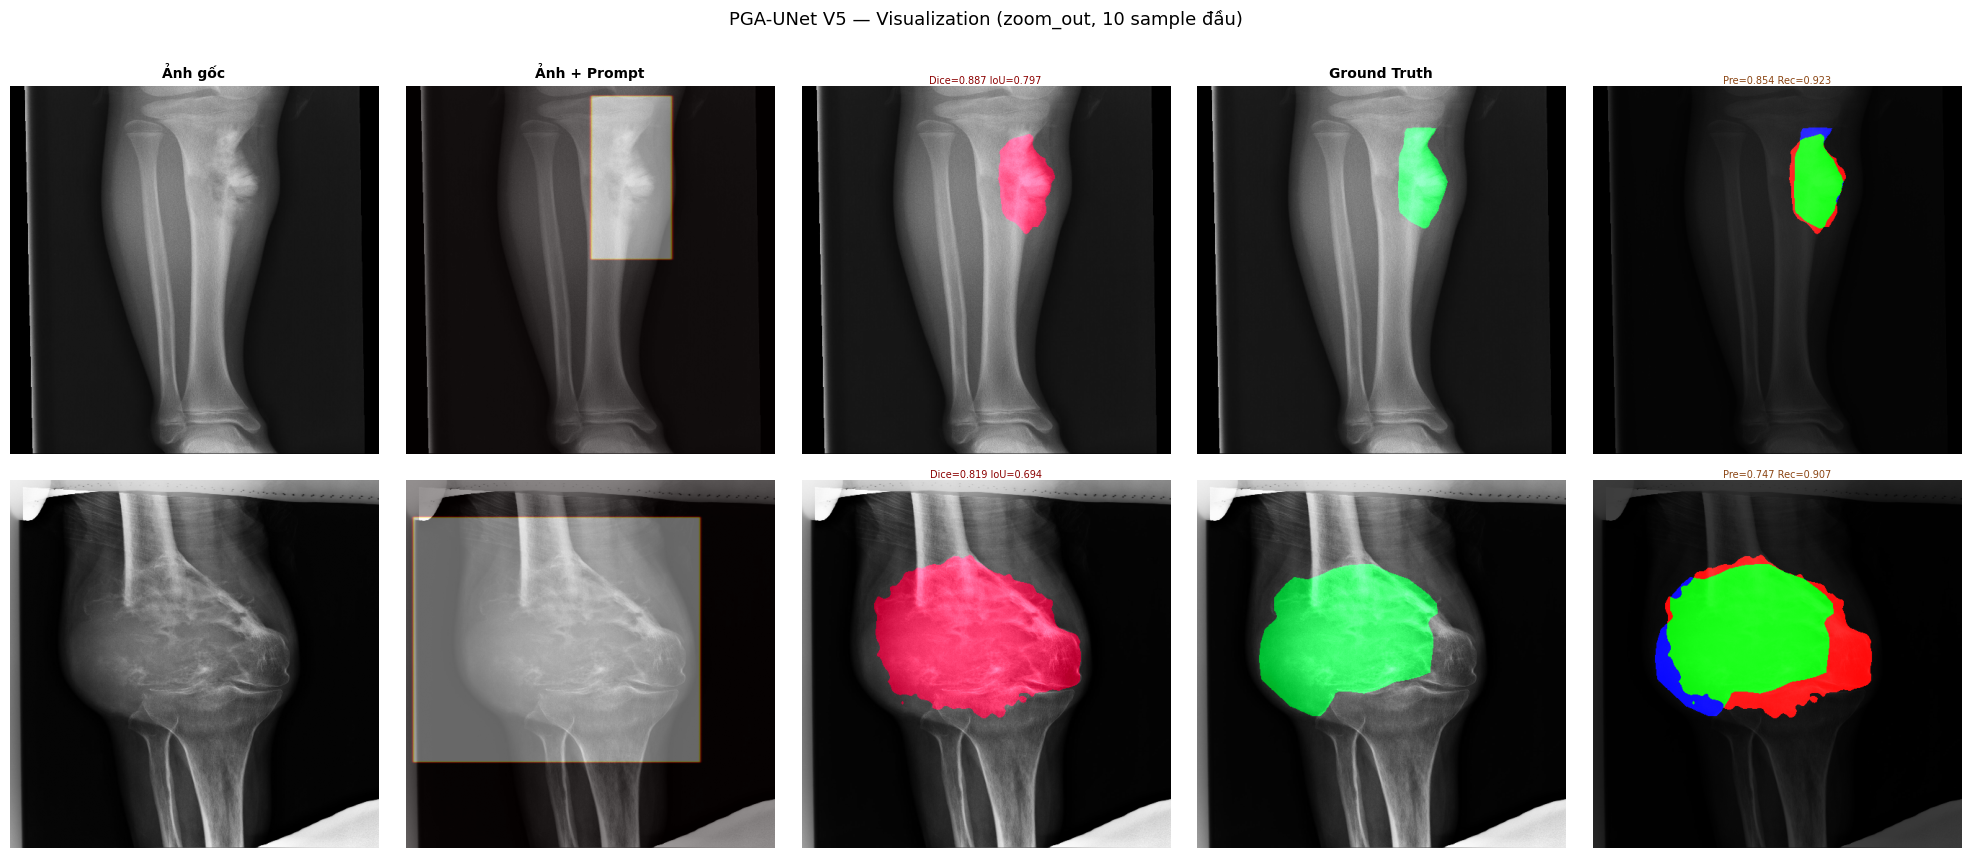
\includegraphics[width=0.95\textwidth]{images/vis_pga_01.png}
    \caption{Kết quả phân đoạn của PGA-UNet trong kịch bản Bao trọn. Từ trái sang phải: ảnh X-quang, hộp giới hạn câu nhắc, mặt nạ dự đoán, mặt nạ nhãn gốc và lớp phủ biểu diễn TP, FP và FN.}
    \label{fig:vis_pga_sample}
\end{figure}

% ------------------------------------------------------------
\subsection{So sánh với mô hình nền tảng SAM-Med2D}
\label{subsec:sam_comparison}
% ------------------------------------------------------------

Trong cấu hình thực nghiệm, SAM-Med2D~\cite{2023-SAMMed2D-Cheng} tiếp nhận ảnh ở kích thước $256\times256$. Để bảo đảm so sánh tại cùng độ phân giải, PGA-UNet được huấn luyện lại từ đầu với kích thước tương ứng trên từng bộ dữ liệu, độc lập với phiên bản $512\times512$ tại Mục~\ref{subsec:baseline_comparison}.

SAM-Med2D được đánh giá ở hai chế độ: chưa tinh chỉnh, sử dụng trực tiếp trọng số tiền huấn luyện; và đã tinh chỉnh, cập nhật lớp thích ứng cùng bộ giải mã trên từng bộ dữ liệu. Các cấu hình sử dụng cùng tập kiểm thử, kịch bản câu nhắc và phương pháp đánh giá cấp độ ảnh tại Mục~\ref{subsec:image_level_eval}.

\begin{table}[H]
    \centering
    \caption{So sánh PGA-UNet với SAM-Med2D trên BTXRD ở độ phân giải $256\times256$ (N=\Ntestimg~ảnh)}
    \label{tab:sam_comparison}
    \renewcommand{\arraystretch}{1.3}
    \resizebox{\textwidth}{!}{%
    \begin{tabular}{|l|l|c|c|c|c|c|c|}
        \hline
        \textbf{Mô hình} & \textbf{Kịch bản} & \textbf{Dice↑} & \textbf{IoU↑} & \textbf{Precision↑} & \textbf{Recall↑} & \textbf{HD95↓ (px)} & \textbf{CBL↑} \\
        \hline
        PGA-UNet & Bao trọn
        & \textbf{0.8433} & \textbf{0.7381} & \textbf{0.8112}
        & \textbf{0.8937} & \textbf{6.34} & \textbf{0.9488} \\
        PGA-UNet & Lệch tâm
        & \textbf{0.8150} & \textbf{0.6982} & \textbf{0.7929}
        & \textbf{0.8574} & \textbf{7.59} & \textbf{0.9267} \\
        PGA-UNet & Hỗn hợp
        & \textbf{0.8344} & \textbf{0.7255} & \textbf{0.8061}
        & \textbf{0.8809} & \textbf{6.73} & \textbf{0.9419} \\
        \hline
        SAM-Med2D (đã tinh chỉnh) & Bao trọn
        & 0.7541 & 0.6385 & 0.7504 & 0.7932 & 11.33 & 0.8949 \\
        SAM-Med2D (đã tinh chỉnh) & Lệch tâm
        & 0.6912 & 0.5645 & 0.6987 & 0.7192 & 12.64 & 0.8564 \\
        SAM-Med2D (đã tinh chỉnh) & Hỗn hợp
        & 0.7334 & 0.6150 & 0.7338 & 0.7687 & 11.79 & 0.8819 \\
        \hline
        SAM-Med2D (chưa tinh chỉnh) & Bao trọn
        & 0.5418 & 0.4002 & 0.4852 & 0.6808 & 17.50 & 0.8409 \\
        SAM-Med2D (chưa tinh chỉnh) & Lệch tâm
        & 0.5266 & 0.3853 & 0.4755 & 0.6591 & 21.12 & 0.8014 \\
        SAM-Med2D (chưa tinh chỉnh) & Hỗn hợp
        & 0.5432 & 0.4002 & 0.4859 & 0.6796 & 17.96 & 0.8318 \\
        \hline
    \end{tabular}%
    }
\end{table}

\begin{table}[H]
    \centering
    \caption{So sánh PGA-UNet với SAM-Med2D trên FracAtlas ở độ phân giải $256\times256$ (N=\NtestimgFA~ảnh)}
    \label{tab:fracatlas_sam_comparison}
    \renewcommand{\arraystretch}{1.3}
    \resizebox{\textwidth}{!}{%
    \begin{tabular}{|l|l|c|c|c|c|c|c|}
        \hline
        \textbf{Mô hình} & \textbf{Kịch bản} & \textbf{Dice↑} & \textbf{IoU↑} & \textbf{Precision↑} & \textbf{Recall↑} & \textbf{HD95↓ (px)} & \textbf{CBL↑} \\
        \hline
        PGA-UNet & Bao trọn
        & \textbf{0.8110} & \textbf{0.6886} & \textbf{0.7790}
        & \textbf{0.8628} & \textbf{3.57} & \textbf{0.9456} \\
        PGA-UNet & Lệch tâm
        & \textbf{0.7842} & \textbf{0.6531} & \textbf{0.7566}
        & \textbf{0.8333} & \textbf{4.02} & \textbf{0.9260} \\
        PGA-UNet & Hỗn hợp
        & \textbf{0.8088} & \textbf{0.6864} & \textbf{0.7801}
        & \textbf{0.8581} & \textbf{3.57} & \textbf{0.9431} \\
        \hline
        SAM-Med2D (đã tinh chỉnh) & Bao trọn
        & 0.7339 & 0.5897 & 0.7358 & 0.7508 & 4.33 & 0.9040 \\
        SAM-Med2D (đã tinh chỉnh) & Lệch tâm
        & 0.6743 & 0.5227 & 0.6715 & 0.6925 & 5.19 & 0.8606 \\
        SAM-Med2D (đã tinh chỉnh) & Hỗn hợp
        & 0.7209 & 0.5745 & 0.7185 & 0.7396 & 4.57 & 0.8916 \\
        \hline
        SAM-Med2D (chưa tinh chỉnh) & Bao trọn
        & 0.5278 & 0.3720 & 0.4854 & 0.6519 & 8.53 & 0.8514 \\
        SAM-Med2D (chưa tinh chỉnh) & Lệch tâm
        & 0.4983 & 0.3460 & 0.4503 & 0.6195 & 9.72 & 0.8098 \\
        SAM-Med2D (chưa tinh chỉnh) & Hỗn hợp
        & 0.5242 & 0.3691 & 0.4858 & 0.6436 & 8.86 & 0.8402 \\
        \hline
    \end{tabular}%
    }
\end{table}

Ở cùng độ phân giải $256\times256$, PGA-UNet cho kết quả cao hơn SAM-Med2D ở cả ba kịch bản trên cả hai bộ dữ liệu. Với câu nhắc Bao trọn, Dice của PGA-UNet cao hơn SAM-Med2D đã tinh chỉnh 0,0892 trên BTXRD và 0,0771 trên FracAtlas. So với SAM-Med2D chưa tinh chỉnh thì khoảng cách còn lớn hơn nữa, lên tới 0,3015 trên BTXRD và 0,2832 trên FracAtlas. Ngoài ra, PGA-UNet cũng có HD95 thấp hơn và CBL lớn hơn 0,94, nghĩa là mặt nạ dự đoán có xu hướng bám vị trí tổn thương tốt hơn trong thiết lập có câu nhắc được kiểm soát. Dù vậy, đây vẫn là kết quả so sánh của hai hệ thống hoàn chỉnh, chưa tách riêng đóng góp của từng thành phần kiến trúc.

Khi chuyển từ câu nhắc Bao trọn sang Lệch tâm, Dice của PGA-UNet giảm 0,0283 trên BTXRD và 0,0268 trên FracAtlas. Mức giảm này nhỏ hơn mức giảm tương ứng của SAM-Med2D đã tinh chỉnh (0,0629 trên BTXRD và 0,0596 trên FracAtlas). Có thể hiểu là trong các kịch bản mô phỏng của khóa luận, PGA-UNet giữ độ ổn định tốt hơn khi câu nhắc không còn lý tưởng nữa.
\begin{figure}[H]
    \centering
    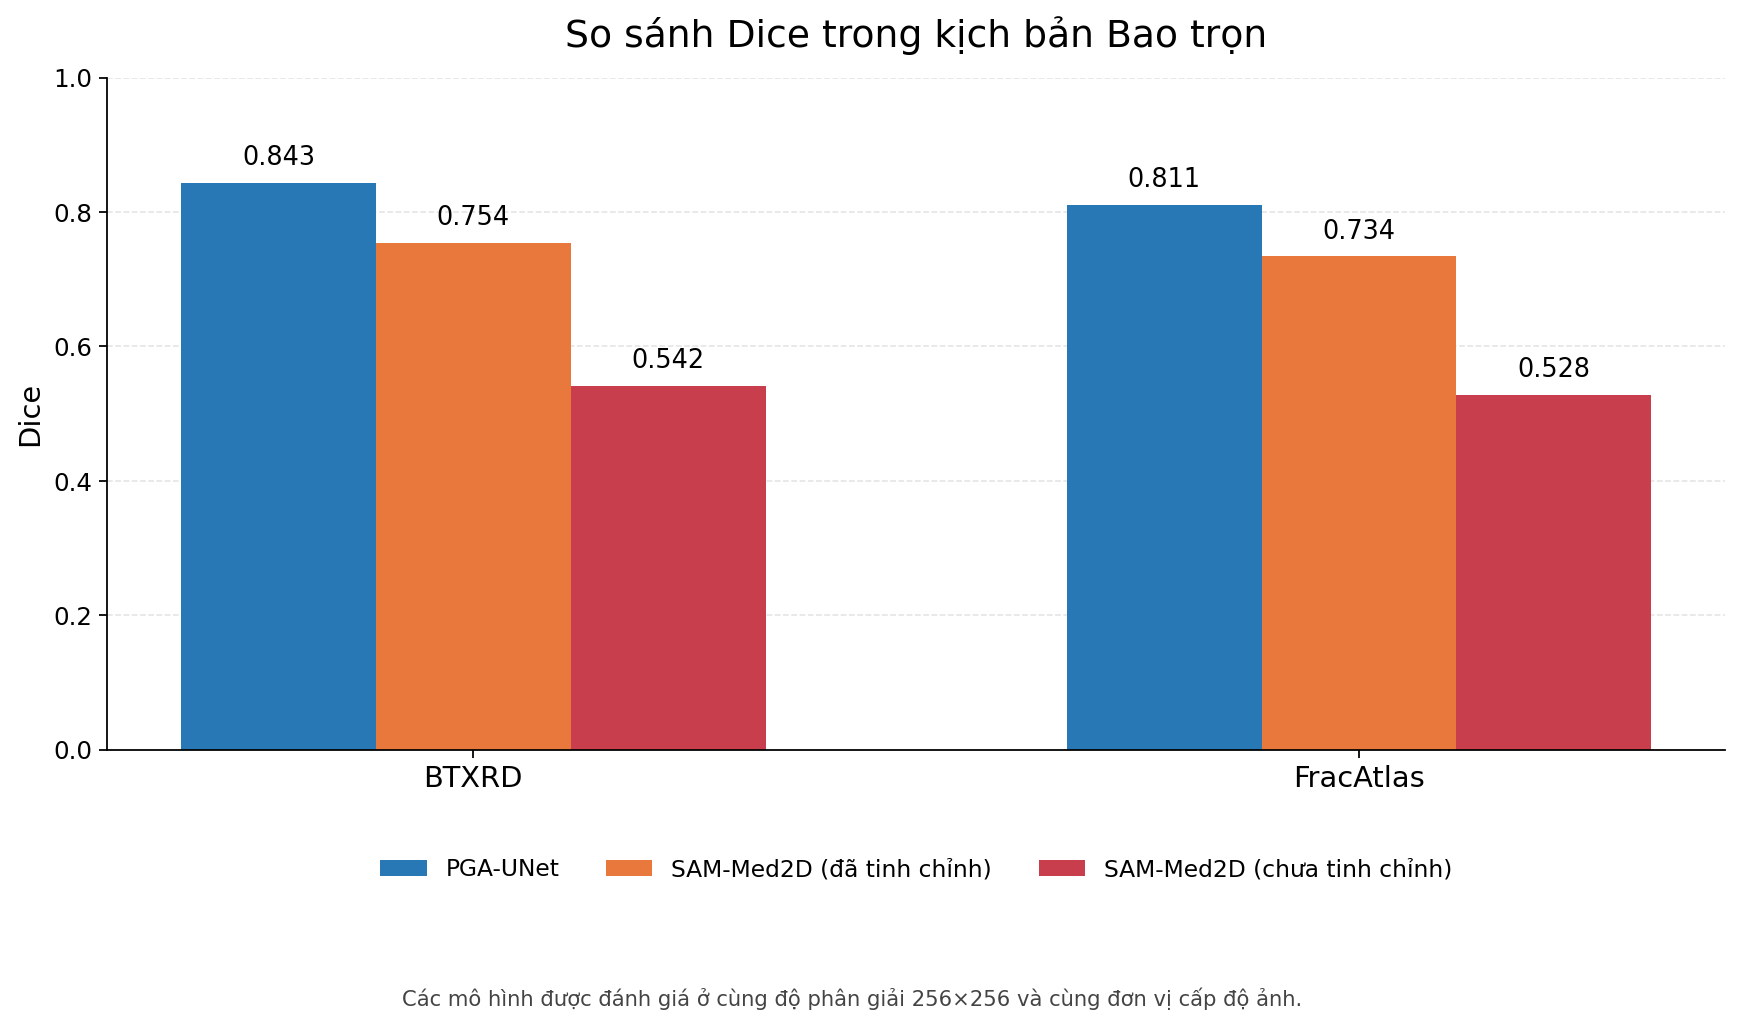
\includegraphics[width=0.75\textwidth]{images/chart_sam_comparison_256.png}
    \caption{So sánh Dice của PGA-UNet và SAM-Med2D trong kịch bản Bao trọn trên BTXRD và FracAtlas. Các cấu hình đều sử dụng độ phân giải $256\times256$ và được đánh giá ở cấp độ ảnh.}
    \label{fig:chart_sam_comparison_combined}
\end{figure}

PGA-UNet được huấn luyện từ đầu trên từng bộ dữ liệu, trong khi SAM-Med2D kế thừa trọng số tiền huấn luyện trên tập ảnh y tế quy mô lớn. Vì vậy, kết quả trên phản ánh hiệu năng của các hệ thống hoàn chỉnh, không tách riêng đóng góp của từng thành phần kiến trúc. Vai trò của PSG và CAD được phân tích tại Mục~\ref{sec:ablation_study} và Phụ lục~\ref{AppendixA}.

% ------------------------------------------------------------
\subsection{Hiệu quả tính toán}
\label{subsec:efficiency_measurement}
% ------------------------------------------------------------

Để phần so sánh không chỉ dừng ở độ chính xác, khóa luận còn đo thêm hiệu quả tính toán của PGA-UNet và SAM-Med2D trong cùng môi trường thực nghiệm. Các chỉ số được ghi nhận gồm số lượng tham số, FLOPs, dung lượng checkpoint, bộ nhớ GPU đỉnh và độ trễ suy luận trung bình. PGA-UNet được đo ở cả $256\times256$ và $512\times512$, còn SAM-Med2D được đo ở $256\times256$, là độ phân giải dùng để đối sánh trực tiếp ở Mục~\ref{subsec:sam_comparison}. Các con số này chỉ mang ý nghĩa so sánh tương đối trong cùng môi trường đo.

Ở cùng độ phân giải $256\times256$, PGA-UNet nhỏ hơn SAM-Med2D khoảng 92 lần về số lượng tham số (2,95M so với 271,24M), khoảng 11,9 lần về FLOPs và nhanh hơn khoảng 7,2 lần trên GPU trong cùng môi trường thực nghiệm. Dung lượng điểm lưu trọng số cũng chênh lệch rất lớn, khoảng 215 lần (11,3 MB so với 2443,2 MB), cho thấy PGA-UNet có chi phí tính toán thấp hơn trong điều kiện đo của khóa luận.

Khi tăng độ phân giải của PGA-UNet lên $512\times512$, FLOPs và độ trễ tăng như kỳ vọng, nhưng mô hình vẫn có độ trễ thấp hơn và dung lượng nhỏ hơn rất nhiều so với SAM-Med2D ở $256\times256$ trong cùng môi trường đo. Bảng số liệu rút gọn và biểu đồ tổng hợp của phép đo này được đưa xuống Phụ lục~\ref{AppendixA}, Mục~\ref{sec:appendix_efficiency}, nhằm giữ cho phần thân bài tập trung vào hai ý chính: trong điều kiện thực nghiệm đã khảo sát, PGA-UNet có chi phí tính toán thấp hơn, trong khi SAM-Med2D đòi hỏi tài nguyên lớn hơn.
% ------------------------------------------------------------
\subsection{Ảnh hưởng của độ phân giải và câu nhắc lệch trong phạm vi bài toán}
\label{subsec:resolution_prompt}
% ------------------------------------------------------------

Mục này khảo sát ảnh hưởng của độ phân giải đầu vào và câu nhắc lệch trong phạm vi bài toán đối với PGA-UNet. Hai phiên bản ở kích thước $256\times256$ và $512\times512$ được huấn luyện độc lập trên từng bộ dữ liệu, sau đó đánh giá trong ba kịch bản Bao trọn, Lệch tâm và Hỗn hợp. Cách tạo các kịch bản câu nhắc được định nghĩa tại Mục~\ref{subsec:training_process} và giữ cố định trong toàn bộ thực nghiệm.

Như đã lưu ý tại Mục~\ref{subsec:models_compared}, kích thước cửa sổ Gaussian ($k=31$) và biên mở rộng hộp giới hạn (5 điểm ảnh) được giữ cố định theo số điểm ảnh đồng thời cho cả hai độ phân giải. Vì vậy, so với kích thước ảnh, câu nhắc ở $256\times256$ được làm mềm và mở rộng tương đối nhiều hơn so với câu nhắc ở $512\times512$. Đây là một yếu tố có thể ảnh hưởng đồng thời cùng với độ phân giải khi so sánh hai cấu hình dưới đây, nên chênh lệch chỉ số Dice giữa hai độ phân giải không chỉ đơn thuần phản ánh độ sắc nét và chi tiết của bức ảnh mà còn chịu ảnh hưởng bởi mức độ tác động tương đối của câu nhắc lên từng độ phân giải.

\begin{table}[H]
    \centering
    \caption{Kết quả PGA-UNet tại hai độ phân giải trên BTXRD (N=\Ntestimg~ảnh)}
    \label{tab:pga_256_512}
    \renewcommand{\arraystretch}{1.3}
    \resizebox{\textwidth}{!}{%
    \begin{tabular}{|c|l|c|c|c|c|c|c|}
        \hline
        \textbf{Độ phân giải} & \textbf{Kịch bản} & \textbf{Dice↑} & \textbf{IoU↑} & \textbf{Precision↑} & \textbf{Recall↑} & \textbf{HD95↓ (px)} & \textbf{CBL↑} \\
        \hline
        $256\times256$ & Bao trọn
        & 0.8433 & 0.7381 & 0.8112 & \textbf{0.8937} & 6.34 & 0.9488 \\
        $256\times256$ & Lệch tâm
        & 0.8150 & 0.6982 & 0.7929 & 0.8574 & 7.59 & 0.9267 \\
        $256\times256$ & Hỗn hợp
        & 0.8344 & 0.7255 & 0.8061 & \textbf{0.8809} & 6.73 & 0.9419 \\
        \hline
        $512\times512$ & Bao trọn
        & \textbf{0.8607} & \textbf{0.7630} & \textbf{0.8476} & 0.8882 & 12.12 & \textbf{0.9564} \\
        $512\times512$ & Lệch tâm
        & \textbf{0.8423} & \textbf{0.7381} & \textbf{0.8405} & \textbf{0.8621} & 14.14 & \textbf{0.9433} \\
        $512\times512$ & Hỗn hợp
        & \textbf{0.8560} & \textbf{0.7567} & \textbf{0.8477} & 0.8803 & 12.62 & \textbf{0.9537} \\
        \hline
    \end{tabular}%
    }
\end{table}

\begin{table}[H]
    \centering
    \caption{Kết quả PGA-UNet tại hai độ phân giải trên FracAtlas (N=\NtestimgFA~ảnh)}
    \label{tab:fracatlas_pga_full}
    \renewcommand{\arraystretch}{1.3}
    \resizebox{\textwidth}{!}{%
    \begin{tabular}{|c|l|c|c|c|c|c|c|}
        \hline
        \textbf{Độ phân giải} & \textbf{Kịch bản} & \textbf{Dice↑} & \textbf{IoU↑} & \textbf{Precision↑} & \textbf{Recall↑} & \textbf{HD95↓ (px)} & \textbf{CBL↑} \\
        \hline
        $256\times256$ & Bao trọn
        & 0.8110 & 0.6886 & \textbf{0.7790} & 0.8628 & 3.57 & 0.9456 \\
        $256\times256$ & Lệch tâm
        & 0.7842 & 0.6531 & \textbf{0.7566} & 0.8333 & 4.02 & 0.9260 \\
        $256\times256$ & Hỗn hợp
        & 0.8088 & 0.6864 & \textbf{0.7801} & 0.8581 & 3.57 & 0.9431 \\
        \hline
        $512\times512$ & Bao trọn
        & \textbf{0.8169} & \textbf{0.6953} & 0.7645 & \textbf{0.8975} & 7.45 & \textbf{0.9546} \\
        $512\times512$ & Lệch tâm
        & \textbf{0.7850} & \textbf{0.6537} & 0.7349 & \textbf{0.8618} & 8.88 & \textbf{0.9308} \\
        $512\times512$ & Hỗn hợp
        & \textbf{0.8129} & \textbf{0.6904} & 0.7614 & \textbf{0.8913} & 7.80 & \textbf{0.9499} \\
        \hline
    \end{tabular}%
    }
\end{table}

\textit{Lưu ý:} HD95 được tính theo đơn vị điểm ảnh tại từng độ phân giải nên không thể so sánh trực tiếp giữa ảnh $256\times256$ và $512\times512$. Vì vậy, các giá trị HD95 không được in đậm trong hai bảng trên.

\begin{figure}[H]
    \centering
    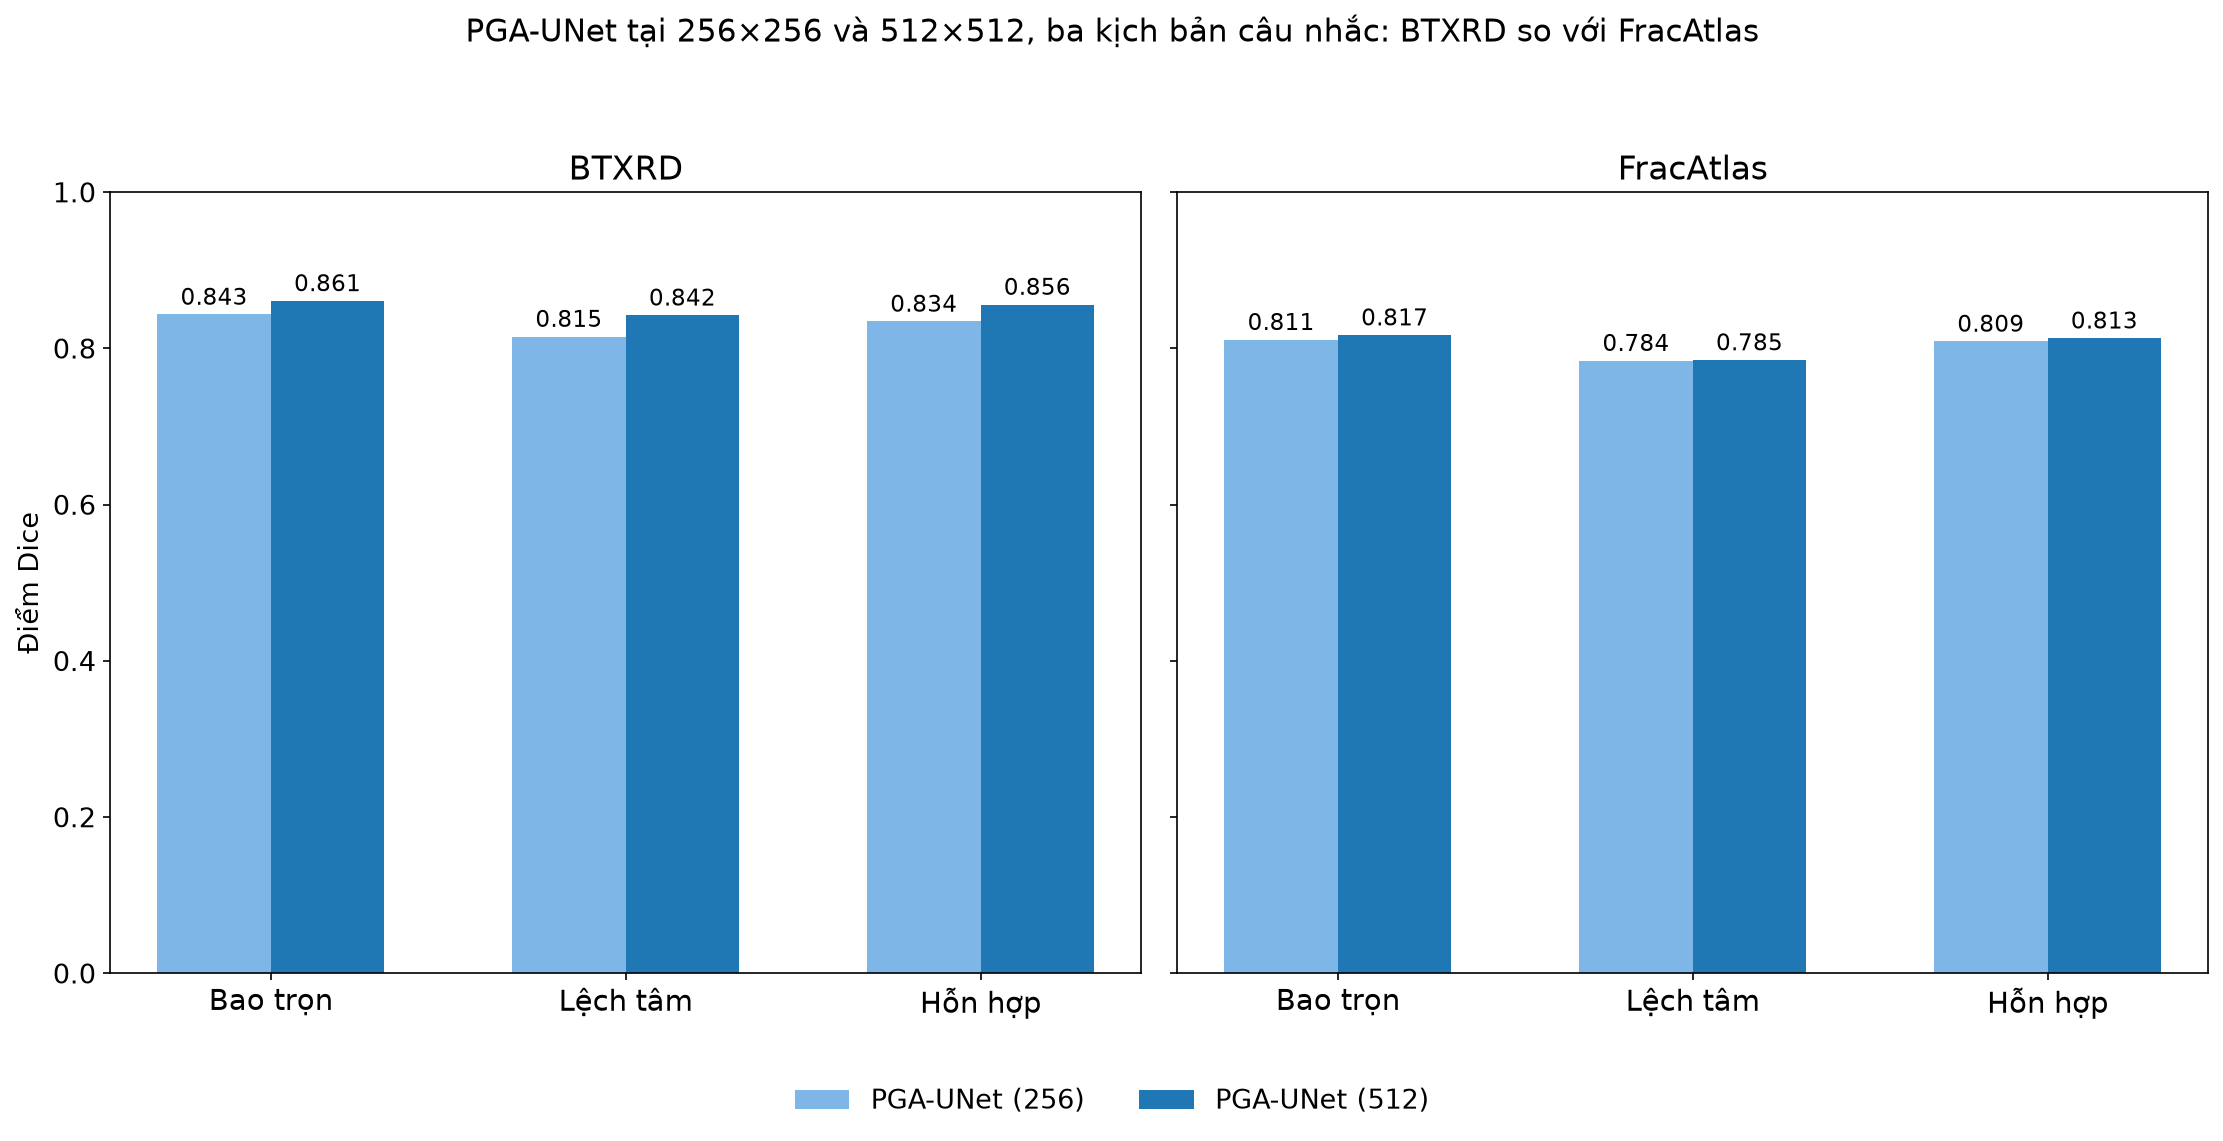
\includegraphics[width=0.95\textwidth]{images/chart_resolution_btxrd_fracatlas.png}
    \caption{Kết quả PGA-UNet tại hai độ phân giải trong ba kịch bản câu nhắc trên BTXRD và FracAtlas.}
    \label{fig:chart_resolution_combined}
\end{figure}

Khi tăng độ phân giải từ $256\times256$ lên $512\times512$, Dice đều tăng ở cả ba kịch bản trên hai bộ dữ liệu, nhưng mức tăng không giống nhau. Trên BTXRD, chênh lệch tăng rõ hơn; còn trên FracAtlas, mức tăng nhỏ hơn nhiều. Một số chỉ số như Precision trên FracAtlas còn giảm nhẹ ở độ phân giải cao hơn. Vì bản đồ câu nhắc cũng thay đổi theo tỉ lệ tương đối giữa hai độ phân giải, nên kết quả này không nên hiểu đơn giản là chỉ do ảnh lớn hơn, mà là tác động tổng hợp của cả độ phân giải ảnh và cách chuẩn hóa câu nhắc.

\vspace{0.5cm}

PGA-UNet duy trì mức suy giảm Dice tương đối nhỏ khi chuyển từ câu nhắc Bao trọn sang Lệch tâm. Mức giảm nằm trong khoảng từ 0,0184 đến 0,0319 trên hai độ phân giải và hai bộ dữ liệu. Kết quả này cần được hiểu là độ ổn định đối với dạng lệch câu nhắc mô phỏng đã khảo sát, không phải khẳng định tổng quát về độ bền vững trước mọi dạng prompt lệch trong thực tế. Khả năng này vẫn cần được kiểm chứng với câu nhắc do bác sĩ chẩn đoán ảnh cung cấp trong thực tế. Cần lưu ý thêm rằng hộp giới hạn Lệch tâm dùng để đánh giá được sinh bằng cùng quy tắc (dịch ngẫu nhiên bằng 0,30 kích thước hộp) đã sử dụng khi huấn luyện, nên kết quả phản ánh độ ổn định của mô hình đối với đúng dạng nhiễu đã học, chưa phải bằng chứng về mức độ lệch chưa từng thấy hoặc do bác sĩ chẩn đoán ảnh thực tế tạo ra.

Hình~\ref{fig:qual_shift} minh họa khả năng dự đoán của PGA-UNet trước câu nhắc Lệch tâm trên một ảnh thuộc mỗi bộ dữ liệu. Trong ví dụ BTXRD, Dice giảm từ 0,922 xuống 0,917; trong ví dụ FracAtlas, Dice giảm từ 0,781 xuống 0,643. Đây là các trường hợp minh họa và không thay thế kết quả trung bình trên toàn bộ tập kiểm thử.

\begin{figure}[H]
    \centering
    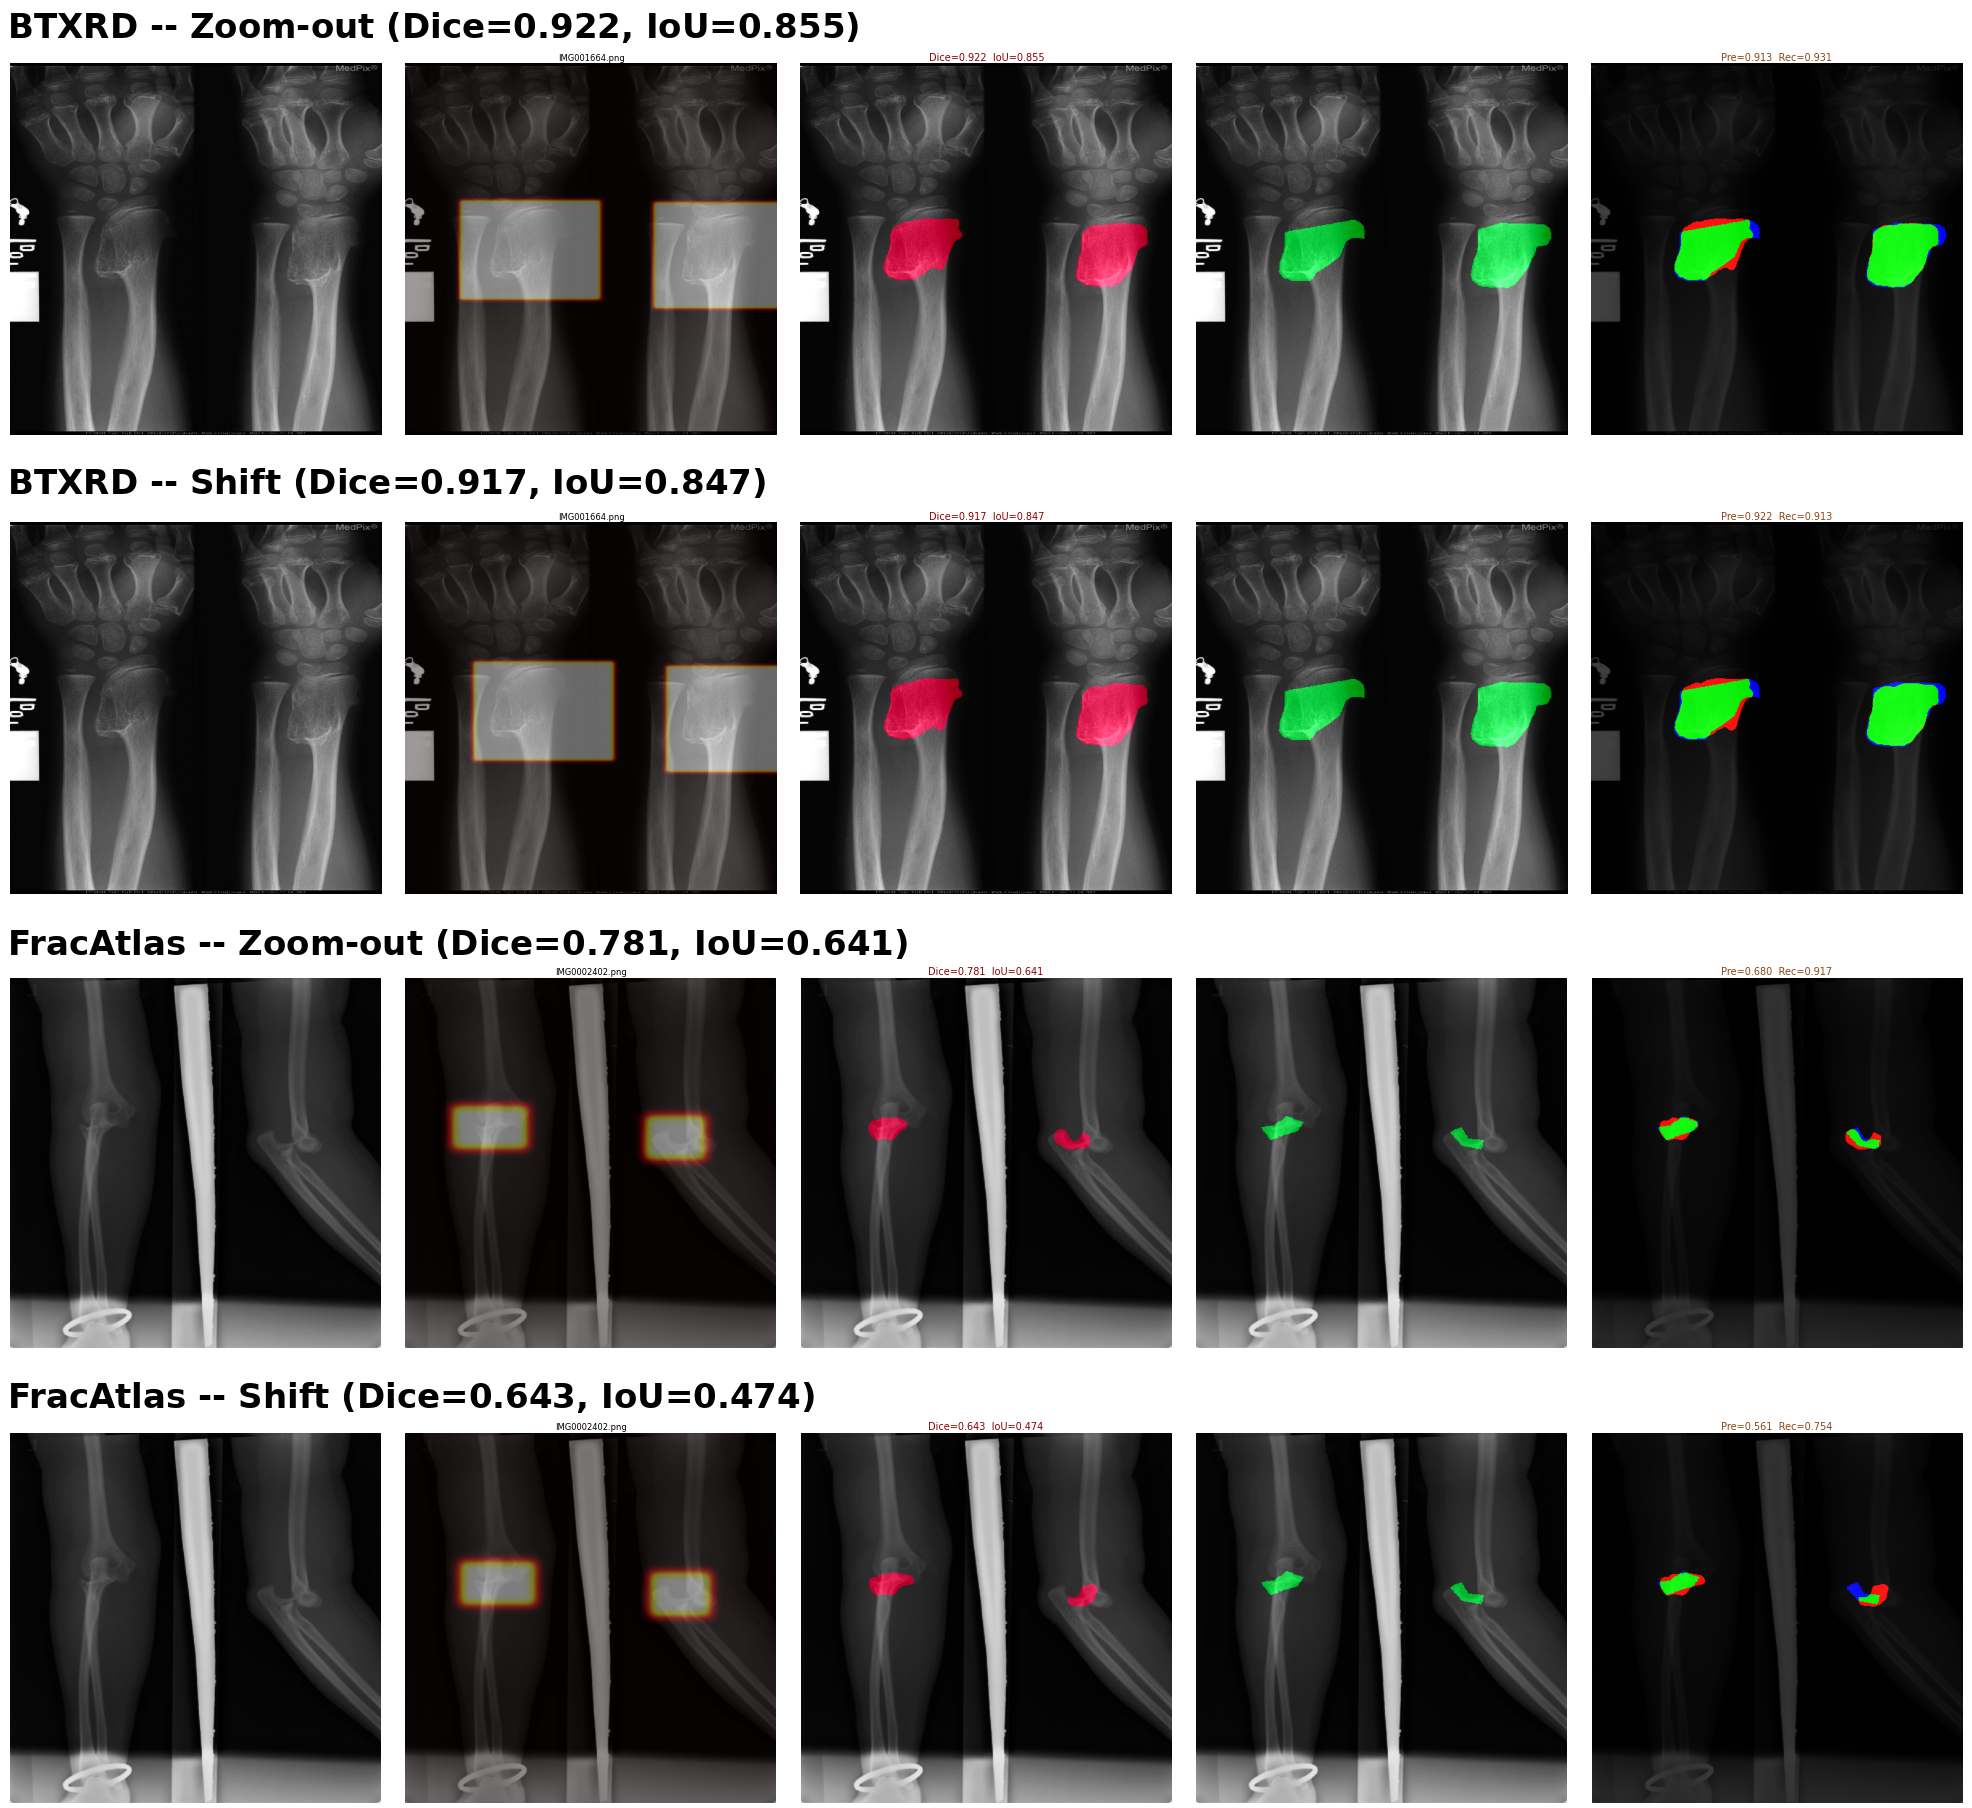
\includegraphics[width=0.9\textwidth]{images/qual_robustness_zoom_shift.png}
    \caption{Kết quả PGA-UNet với câu nhắc Bao trọn và Lệch tâm trên BTXRD (hàng trên) và FracAtlas (hàng dưới).}
    \label{fig:qual_shift}
\end{figure}

% ============================================================
\section{Tổng hợp đóng góp kiến trúc và tính nhất quán trên hai bộ dữ liệu}
\label{sec:ablation_study}
% ============================================================

Bên cạnh các phép so sánh chính, khóa luận còn làm thêm ba nhóm thực nghiệm bổ sung để xem đóng góp của từng thành phần kiến trúc rõ đến đâu. Ba nhóm đó gồm nghiên cứu loại bỏ thành phần, kiểm chứng chéo 4 lần và phân tích theo đặc tính tổn thương. Các thí nghiệm này được thực hiện độc lập trên cả BTXRD và FracAtlas. Trong mục này chỉ tóm tắt các kết luận quan trọng nhất; số liệu đầy đủ và hình minh họa bổ sung được để ở Phụ lục~\ref{AppendixA}.

% ------------------------------------------------------------
\subsection{Đóng góp của PSG, CAD và bản đồ nhiệt Gaussian}
\label{subsec:summary_ablation}
% ------------------------------------------------------------

Tám cấu hình, tổ hợp giữa không hoặc có PSG, ba lựa chọn cho cơ chế chú ý trên các kết nối tắt của nhánh giải mã (không cổng chú ý, cổng chú ý nguyên bản của Attention U-Net~\cite{oktay2018attentionunet}, hoặc CAD) và hai cách biểu diễn câu nhắc (nhị phân hoặc Gaussian), được huấn luyện lại từ đầu trên cùng dữ liệu và cùng điều kiện huấn luyện của BTXRD và FracAtlas. U-Net+Concat, chỉ nối câu nhắc vào ảnh đầu vào, đóng vai trò cấu hình cơ sở cùng nhận câu nhắc như PGA-UNet.

\begin{table}[H]
    \centering
    \caption{Tổng hợp Dice của ba cấu hình chính trong nghiên cứu loại bỏ thành phần trên BTXRD và FracAtlas (ba kịch bản câu nhắc)}
    \label{tab:ablation_summary}
    \renewcommand{\arraystretch}{1.3}
    \resizebox{\textwidth}{!}{%
    \begin{tabular}{|l|c|c|c|c|c|c|}
        \hline
        \multirow{2}{*}{\textbf{Cấu hình}}
        & \multicolumn{3}{c|}{\textbf{BTXRD}}
        & \multicolumn{3}{c|}{\textbf{FracAtlas}} \\
        \cline{2-7}
        & \textbf{Bao trọn↑} & \textbf{Lệch tâm↑} & \textbf{Hỗn hợp↑}
        & \textbf{Bao trọn↑} & \textbf{Lệch tâm↑} & \textbf{Hỗn hợp↑} \\
        \hline
        U-Net+Concat (Gaussian, cơ sở có câu nhắc)
        & 0.8763 & 0.7364 & 0.8216
        & 0.8131 & 0.6579 & 0.7573 \\
        \hline
        Cấu hình tốt nhất ở Bao trọn
        & \textbf{0.8861} & 0.7406 & 0.8292
        & \textbf{0.8351} & 0.6927 & 0.7838 \\
        \hline
        \textbf{PGA-UNet}
        & 0.8607 & \textbf{0.8423} & \textbf{0.8560}
        & 0.8169 & \textbf{0.7850} & \textbf{0.8129} \\
        \hline
    \end{tabular}%
    }
    \vspace{2pt}
    \\
    \footnotesize Cấu hình đạt Dice cao nhất ở kịch bản Bao trọn trong tám cấu hình khảo sát: U-Net+CAD trên BTXRD, U-Net+PSG+Cổng chú ý nguyên bản trên FracAtlas. Toàn bộ tám cấu hình được trình bày tại Bảng~\ref{tab:ablation_arch} và~\ref{tab:fracatlas_ablation_arch}, Phụ lục~\ref{AppendixA}.
\end{table}

Bảng~\ref{tab:ablation_summary} cho thấy một xu hướng rõ ràng trên cả hai bộ dữ liệu. PGA-UNet không phải cấu hình có Dice cao nhất trong kịch bản Bao trọn (thấp hơn cấu hình tốt nhất 0,0254 trên BTXRD và 0,0182 trên FracAtlas), nhưng lại là cấu hình tốt nhất ở hai kịch bản Lệch tâm và Hỗn hợp. Nói ngắn hơn, điểm mạnh chính của mô hình không nằm ở trường hợp câu nhắc quá đẹp, mà nằm ở khả năng giữ kết quả ổn hơn khi câu nhắc bị lệch như trong các tình huống mô phỏng của khóa luận.

Để kiểm tra độ tin cậy của xu hướng trên ở cấp độ ảnh, sáu cặp cấu hình được kiểm định bằng Wilcoxon signed-rank trên Dice bắt cặp theo từng ảnh, thực hiện riêng trên hai bộ dữ liệu và ba kịch bản (36 kết quả, giá trị $p$ thô, chưa hiệu chỉnh cho so sánh nhiều lần). Hai phát hiện có bằng chứng mạnh và nhất quán nhất trên cả hai bộ dữ liệu đều thuộc kịch bản Lệch tâm:
\begin{itemize}
    \item Thay cổng chú ý nguyên bản (đã có PSG) bằng CAD làm Dice tăng 0,1065 trên BTXRD và 0,0924 trên FracAtlas, cả hai đều đạt $p<0{,}001$.
    \item Thay câu nhắc nhị phân bằng bản đồ nhiệt Gaussian (trong cấu hình đầy đủ PSG+CAD) làm Dice tăng 0,0990 trên BTXRD và 0,1005 trên FracAtlas, cả hai đều đạt $p<0{,}001$.
\end{itemize}

Đây là hai bằng chứng thống kê nhất quán và mạnh nhất cho vai trò của CAD và bản đồ nhiệt Gaussian đối với khả năng duy trì hiệu năng dưới mô phỏng lệch câu nhắc. Ngược lại, khi PSG hoặc CAD được sử dụng riêng lẻ (không kết hợp với thành phần còn lại), mức cải thiện so với U-Net+Concat đều nhỏ hơn 0,02 Dice và không nhất quán chiều giữa hai bộ dữ liệu; các thành phần riêng lẻ vì vậy không được xem là quy luật kiến trúc chung. Toàn bộ tám cấu hình, phân tích theo từng thành phần trên từng bộ dữ liệu và bảng kiểm định Wilcoxon đầy đủ (36 kết quả) được trình bày tại Mục~\ref{subsec:ablation_arch}, \ref{subsec:fracatlas_ablation} và \ref{subsec:conclusion_arch}, Phụ lục~\ref{AppendixA}.

% ------------------------------------------------------------
\subsection{Độ ổn định qua các phân vùng dữ liệu}
\label{subsec:summary_cv}
% ------------------------------------------------------------

PGA-UNet cũng được đánh giá bằng kiểm chứng chéo ngẫu nhiên lặp lại trên cả BTXRD và FracAtlas, trong đó các đa giác thuộc cùng một ảnh luôn được giữ trong cùng một phân vùng. Trên BTXRD, độ lệch chuẩn của Dice qua bốn phân vùng nằm trong khoảng 0,0087 đến 0,0119; còn trên FracAtlas là 0,0064 đến 0,0084. Giá trị Dice trung bình giữa các phân vùng cũng sát với kết quả trên tập kiểm thử độc lập.

Độ lệch chuẩn tương đối thấp trên cả hai bộ dữ liệu cho thấy PGA-UNet tương đối ổn định trước các cách chia dữ liệu đã khảo sát. Các bảng chi tiết hơn được để ở Phụ lục~\ref{AppendixA}.

% ------------------------------------------------------------
\subsection{Hiệu năng theo đặc tính tổn thương}
\label{subsec:summary_subcat}
% ------------------------------------------------------------

PGA-UNet được đối chiếu với U-Net và SAM-Med2D trên các nhóm ảnh phân theo đặc tính tổn thương (kích thước, độ rõ đường biên) trên cả hai bộ dữ liệu. Trong các nhóm được khảo sát, khoảng cách Dice giữa PGA-UNet và mô hình SAM-Med2D ở nhóm tổn thương nhỏ (BTXRD: PGA-UNet cao hơn SAM-Med2D 0,5514 Dice; FracAtlas: cao hơn khoảng 0,319), thu hẹp dần và gần bằng nhau hơn ở nhóm tổn thương có hình thái rõ ràng (BTXRD: chênh lệch còn 0,0131; FracAtlas: còn khoảng 0,068). Khi so sánh với U-Net trên các ảnh mà U-Net hoạt động kém, xu hướng tương tự cũng xuất hiện trên cả hai bộ dữ liệu: ở nhóm BOTTOM-DICE (ảnh U-Net dự đoán kém nhất), U-Net đạt Dice rất thấp (BTXRD $=0,0211$; FracAtlas $=0,1130$), trong khi PGA-UNet vẫn đạt trên 0,80 ở cả hai bộ dữ liệu (BTXRD $0,8261$; FracAtlas $0,8015$).

Một trong ba nhóm phân tích (``Biên mờ'') được xác định dựa trên chính Dice thấp của SAM-Med2D trên từng bộ dữ liệu, nên chỉ mang tính mô tả, không phải một phép kiểm định độc lập về độ khó của tổn thương. Toàn bộ bảng số liệu, biểu đồ và hình ảnh định tính theo từng nhóm được trình bày tại Mục~\ref{subsec:subcategory} và~\ref{subsec:fracatlas_subcat}, Phụ lục~\ref{AppendixA}.

\noindent\textbf{Các trường hợp còn hạn chế.}
Qua quan sát định tính trên tập kiểm thử, PGA-UNet vẫn đạt Dice thấp trên một số tổn thương có hình dạng kéo dài hoặc phân nhánh, tổn thương nằm tại vùng giải phẫu chồng lấp (vai, xương đòn, cổ chân), hoặc trên ảnh có độ tương phản thấp. Hình~\ref{fig:qual_overlap} minh họa một trường hợp tổn thương tại vùng vai, xương đòn và lồng ngực chồng lấp, nơi mô hình chỉ đạt Dice 0,762 dù hộp giới hạn đã bao phủ đúng vùng tổn thương.

\begin{figure}[H]
    \centering
    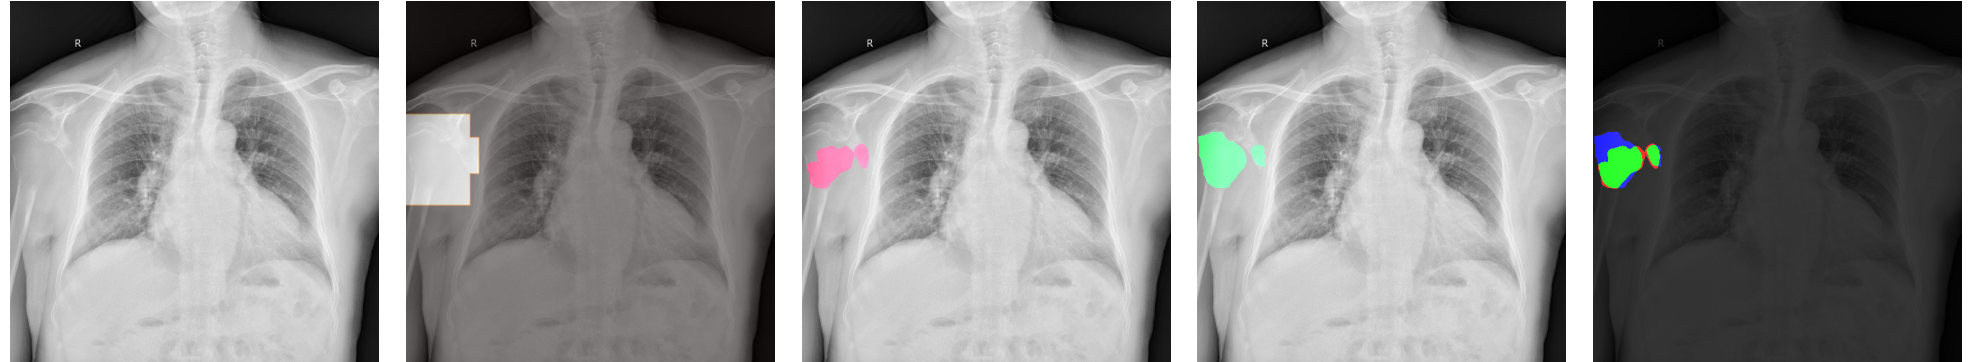
\includegraphics[width=0.75\textwidth]{images/qual_overlap_case.png}
    \caption{Trường hợp tổn thương tại vùng giải phẫu chồng lấp ở vai, xương đòn và lồng ngực, với Dice đạt 0,762.}
    \label{fig:qual_overlap}
\end{figure}

Các nhóm khó nêu trên được nhận diện bằng quan sát định tính, chưa được bác sĩ chẩn đoán ảnh xác nhận hoặc kiểm định thống kê độc lập; chúng chỉ mô tả những tình huống mô hình còn gặp khó khăn, phù hợp với các hạn chế được tổng hợp tại Chương~\ref{Chapter5}.

% ------------------------------------------------------------
\subsection{Kết luận về phạm vi đóng góp kiến trúc}
\label{subsec:conclusion_arch_summary}
% ------------------------------------------------------------

Kết quả nhất quán nhất trên cả BTXRD và FracAtlas là vai trò của CAD và bản đồ nhiệt Gaussian đối với khả năng duy trì hiệu năng khi câu nhắc bị lệch tâm, được xác nhận bằng kiểm định Wilcoxon với $p<0{,}001$ trên cả hai bộ dữ liệu. PGA-UNet được huấn luyện lại độc lập trên từng bộ dữ liệu và duy trì cùng xu hướng trên cả tổn thương khối u xương lẫn đường gãy xương, cung cấp bằng chứng về khả năng tái lập của thiết kế trên hai miền dữ liệu độc lập; đây chưa phải tổng quát hóa liên miền theo nghĩa huấn luyện trên một bộ dữ liệu rồi suy luận trực tiếp trên miền chưa từng thấy.

Các thành phần riêng lẻ (PSG hoặc CAD khi đứng một mình) có biên độ ảnh hưởng nhỏ và không nhất quán giữa hai bộ dữ liệu, nên không được diễn giải như một quy luật kiến trúc tổng quát. Phạm vi kết luận của mục này giới hạn ở mô-đun phân đoạn; khả năng hoạt động của toàn bộ hệ thống, bao gồm tầng sàng lọc đầu vào, được đánh giá riêng tại Mục~\ref{sec:product_overview}. Phần chứng minh đầy đủ cho các kết luận trên, bao gồm bảng Wilcoxon 36 kết quả và toàn bộ số liệu theo từng cấu hình, được trình bày tại Mục~\ref{subsec:conclusion_arch}, Phụ lục~\ref{AppendixA}.

% ------------------------------------------------------------
\section{Đánh giá luồng xử lý hỗ trợ hai giai đoạn}
\label{sec:product_overview}
% ------------------------------------------------------------

Để minh họa cách PGA-UNet có thể được dùng trong một quy trình lớn hơn, khóa luận thực hiện một thử nghiệm mở rộng bằng cách đặt Gatekeeper (EfficientNet-B3~\cite{tan2019efficientnet}) trước PGA-UNet. Vai trò của Gatekeeper là phân loại ảnh thành bình thường hoặc nghi ngờ có bất thường trước khi đi tiếp sang bước phân đoạn. Thực nghiệm này không nhằm giới thiệu một hệ thống lâm sàng hoàn chỉnh, mà chỉ muốn cho thấy lỗi sàng lọc ở bước đầu có thể ảnh hưởng thế nào đến mô-đun phân đoạn ở bước sau. Toàn bộ số liệu chi tiết được để ở Phụ lục~\ref{AppendixB}.

Trên BTXRD, Gatekeeper đạt AUC-ROC 0,9421, Sensitivity 89,30\% và Specificity 86,17\%. Khi kết quả Gatekeeper được sử dụng trực tiếp không qua hiệu chỉnh của bác sĩ chẩn đoán ảnh, 20/187 ảnh bệnh lý bị loại nhầm; Dice toàn luồng có phạt lỗi sàng lọc giảm từ 0,8626 (trên ảnh được sàng lọc đúng) xuống 0,6763. Trên FracAtlas, do dữ liệu mất cân bằng hơn (72/409 ảnh bệnh lý), Gatekeeper chỉ đạt Sensitivity 70,83\% dù Specificity vẫn cao (91,99\%); Dice toàn luồng giảm còn 0,4230, thấp hơn nhiều so với Dice 0,8169 của PGA-UNet khi được đánh giá độc lập trên toàn bộ tập kiểm thử bệnh lý.

Kết quả trên cả hai bộ dữ liệu cho thấy sai số tại bước sàng lọc có thể làm giảm đáng kể hiệu năng toàn luồng, đặc biệt khi dữ liệu mất cân bằng. Vì vậy, Gatekeeper chỉ nên đóng vai trò hỗ trợ ưu tiên ca nghi ngờ; quyết định chuyển bước và cung cấp câu nhắc vẫn cần sự xác nhận của bác sĩ chẩn đoán ảnh, đúng theo cơ chế \textit{sàng lọc mềm} đã trình bày tại Mục~\ref{sec:phan_lop}, Chương~\ref{Chapter3}.
% ------------------------------------------------------------
\section{Tổng kết chương}
\label{sec:summary_ch4}
% ------------------------------------------------------------

Chương này đã trình bày toàn bộ phần thực nghiệm của PGA-UNet trên BTXRD và FracAtlas, gồm so sánh với các mô hình cơ sở, so sánh với SAM-Med2D, khảo sát ảnh hưởng của độ phân giải và tổng hợp kết quả từ nghiên cứu loại bỏ thành phần, kiểm chứng chéo và phân tích theo đặc tính tổn thương. Trong phạm vi phân đoạn có hướng dẫn bằng hộp giới hạn, PGA-UNet cho kết quả tốt hơn các mô hình cơ sở không dùng câu nhắc và cũng cao hơn SAM-Med2D trong phép so sánh cùng điều kiện ở độ phân giải $256\times256$. Mô hình cũng giữ được độ ổn định tốt hơn dưới các mô phỏng lệch câu nhắc.

Kết quả nghiên cứu loại bỏ thành phần cho thấy hiệu quả của mô hình đến từ sự phối hợp giữa PSG, CAD và bản đồ nhiệt Gaussian, trong đó CAD và bản đồ nhiệt Gaussian là hai phần nổi bật hơn ở khả năng chịu lệch câu nhắc. Khi huấn luyện lại trên FracAtlas, xu hướng kết quả chính vẫn được giữ, nghĩa là thiết kế của PGA-UNet giữ được sự nhất quán nhất định trên hai bộ dữ liệu khảo sát. Các bảng số liệu chi tiết hơn được trình bày ở Phụ lục~\ref{AppendixA}.

Thử nghiệm mở rộng với Gatekeeper cho thấy bước sàng lọc có thể hữu ích nếu muốn đặt PGA-UNet trong một luồng xử lý ảnh hỗn hợp. Tuy nhiên, sai số ở bước này cũng có thể kéo hiệu năng toàn luồng giảm đáng kể. Vì vậy, Gatekeeper chỉ nên được dùng như công cụ hỗ trợ, còn việc chuyển bước và cung cấp câu nhắc vẫn cần bác sĩ chẩn đoán ảnh xác nhận.

Nhìn chung, phần thực nghiệm làm rõ thêm rằng đóng góp chính của khóa luận nằm ở kiến trúc PGA-UNet và cách khai thác câu nhắc thông qua PSG, CAD và bản đồ nhiệt Gaussian. Những hạn chế còn lại và hướng phát triển tiếp theo được trình bày ở Chương~\ref{Chapter5}.
